\chapter{Event Categorisation}
\label{chap:event_select}

\newpage
\section{Introduction}


\section{The Diphoton BDT}


\section{Top Fusion Tag}

\subsection{Leptonic}
\subsection{Hadronic}


\section{Associated Production Tag}

\subsection{Leptonic}
\subsection{Hadronic}
\subsection{MET}


\section{Vector Boson Fusion Tag}

\subsection{Introduction}
\subsection{Legacy Tag}
\subsection{Jet Images}

\begin{figure}[h!]

    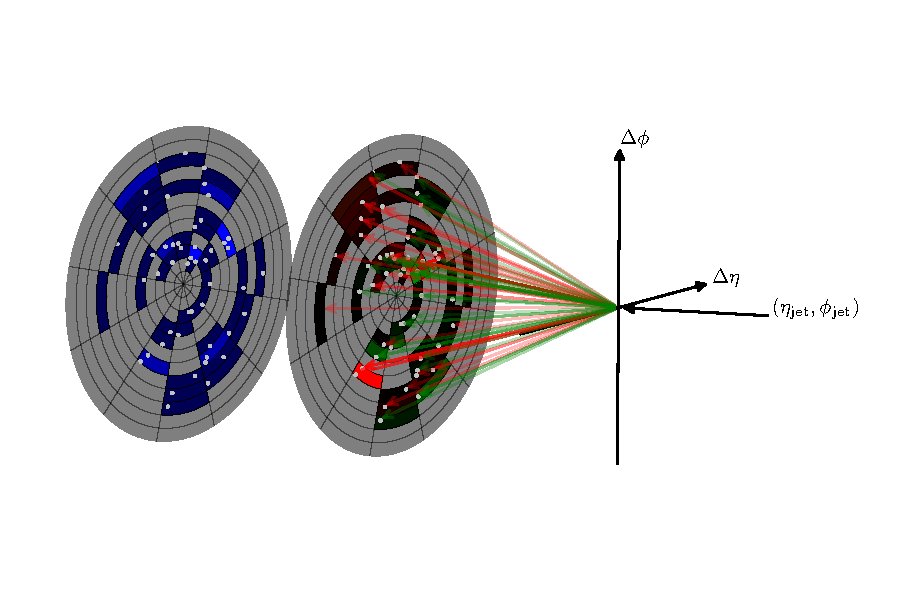
\includegraphics[width=\textwidth]{figures/event_selection/jet_diagram_RGB.pdf}
    \begin{center}
        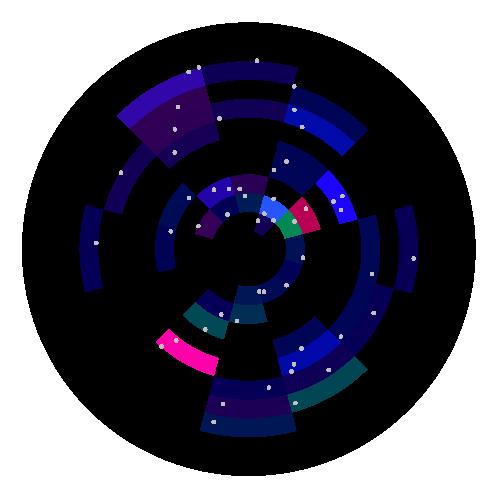
\includegraphics[width=0.49\textwidth]{figures/event_selection/full_image_polar.pdf}
        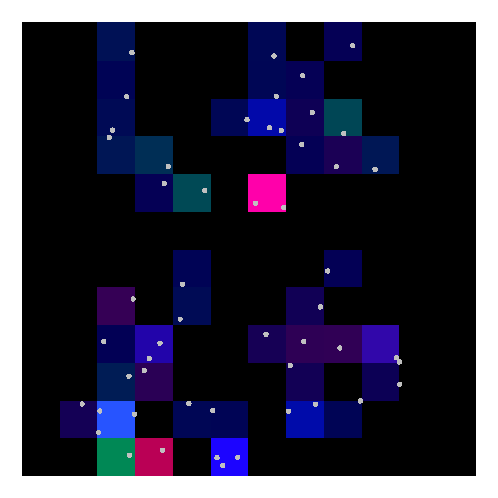
\includegraphics[width=0.49\textwidth]{figures/event_selection/full_image_rect.pdf}
    \end{center}

    \caption{\textbf{Top:} construction of single-jet image from jet constituents. Arrows correspond to individial PF candidates where red arrows are charged, green are neutral and the opacity corresponds to $p_{T}$.
             The red channel measures charged candidate $p_T$ deposition in each pixel, 
             the green channel is neutral charged candidates $p_T$ deposition, 
             and the blue channel is the number of candidates in each pixel (multiplicity). 
             Multiplicity channel is drawn separately so the charged and neutral channels can be seen clearly. Black pixels are lightened to show coloured pixels more clearly.\\
             \textbf{Bottom:} the final image with all the channels together.}
        \label{fig:event_categorisatoin:jet_image}
\end{figure}


\subsection{Model Architecture}
\subsection{Training}
\subsection{Model Optimisation}
\subsection{Model Evaluation}
\subsection{Boundary Optimisation}

\section{Untagged}
